\section{Построение фронтов Парето для различных управляющих структур}

Наличие нескольких критериев оптимизации требует решения вопроса выбора
предпочтительной структуры на основании сравнения фронтов Парето, построенных
для каждой конкурсной структуры. Использование традиционных методов построения
множества Парето приводит к необходимости проведения многократных расчетов с
использованием сложных динамических моделей. Это существенно увеличивает трудоемкость
процесса получения решения и делает процесс затратным по времени.

Для решения этой проблемы было предложено использование замещающих суррогатных
моделей (surrogate models) \cite{surrogate_model} при построении фронтов Парето.
Данные модели строятся на основании исходных моделей и способны с достаточной
точностью аппроксимировать зависимость критериев оптимизации от параметров
пневмопривода. Основная цель использования суррогатных
моделей заключается в снижении вычислительных затрат при поиске Парето-оптимальных
решений за счёт замены трудоёмкого полного моделирования более быстрой аппроксимацией

Проведенный анализ (приложение \ref{app:choosing-the-best-surrogate-model-method}) показал,
что наиболее предпочтительно в качестве суррогатной модели использовать нейронную сеть с
глубокой архитектурой, включающей остаточные связи (residual connections)
для улучшения сходимости при обучении. Основным строительным
блоком такой сети является резидуальный блок, описываемый следующими уравнениями \cite{he2015deepresiduallearningimage}:

\begin{equation}
	\mathbf{h}_1 = \phi(\mathbf{W}_1 \mathbf{x} + \mathbf{b}_1),
\end{equation}
\begin{equation}
	\mathbf{h}_2 = \mathbf{W}_2 \mathbf{D}(\mathbf{h}_1) + \mathbf{b}_2,
\end{equation}
\begin{equation}
	\mathbf{y} = \phi(\mathbf{h}_2 + \mathbf{W}_s \mathbf{x}),
\end{equation}
где $\mathbf{x}$ -- входной вектор параметров управляющей структуры;
$\mathbf{W}_1, \mathbf{W}_2, \mathbf{W}_s$ -- весовые матрицы;
$\mathbf{b}_1, \mathbf{b}_2$ -- векторы смещения;
$\phi(\cdot)$ -- функция активации (ReLU);
$\mathbf{D}(\cdot)$ -- функция прореживания (Dropout) с вероятностью \num{0.1};
$\mathbf{y}$ -- выходной вектор резидуального блока.
\nomenclature{$\mathbf{x}$}{Вектор параметров управляющей структуры\nomrefeqpage}
\nomenclature{$\mathbf{y}$}{вектор резидуального блока\nomrefeqpage}
\nomenclature{$\mathbf{h}_1$}{Выходной вектор первого резидуального блока\nomrefeqpage}
\nomenclature{$\mathbf{h}_2$}{Выходной вектор второго резидуального блока\nomrefeqpage}
\nomenclature{$\mathbf{W}_1, \mathbf{W}_2, \mathbf{W}_s$}{Весовые матрицы\nomrefeqpage}
\nomenclature{$\mathbf{b}_1, \mathbf{b}_2$}{Векторы смещения\nomrefeqpage}
\nomenclature{$\phi(\cdot)$}{Функция активации\nomrefeqpage}
\nomenclature{$\mathbf{D}(\cdot)$}{Функция прореживания\nomrefeqpage}


Полная архитектура суррогатной модели включает последовательность резидуальных блоков
с увеличением размерности скрытых слоёв и заключительный линейный слой
для предсказания значений критериев оптимизации:

\begin{equation}
	\mathbf{y} = f(\mathbf{x}) = \mathbf{W}_\text{out} \cdot \text{RB}_n(\text{RB}_{n-1}(...\text{RB}_1(\mathbf{x})...)) + \mathbf{b}_\text{out},
\end{equation}
где $\text{RB}_i$ -- $i$-й резидуальный блок;
$\mathbf{W}_\text{out}, \mathbf{b}_\text{out}$ -- параметры выходного слоя;
$n$ -- количество резидуальных блоков, определяемое в процессе оптимизации гиперпараметров.

Использование нейросетевых суррогатных моделей при построении фронтов Парето
требует решения вопросов предварительного обучения нейросети на основании серии
расчетов по исходной модели (рисунок \ref{fig:process-diagram}). Для этого в пространстве
параметров формируется выборка данных (расчетные точки) на основании
которых в результате численного моделирования по исходной модели
рассчитываются показатели качества.

\begin{figure}[h]
	\centering
	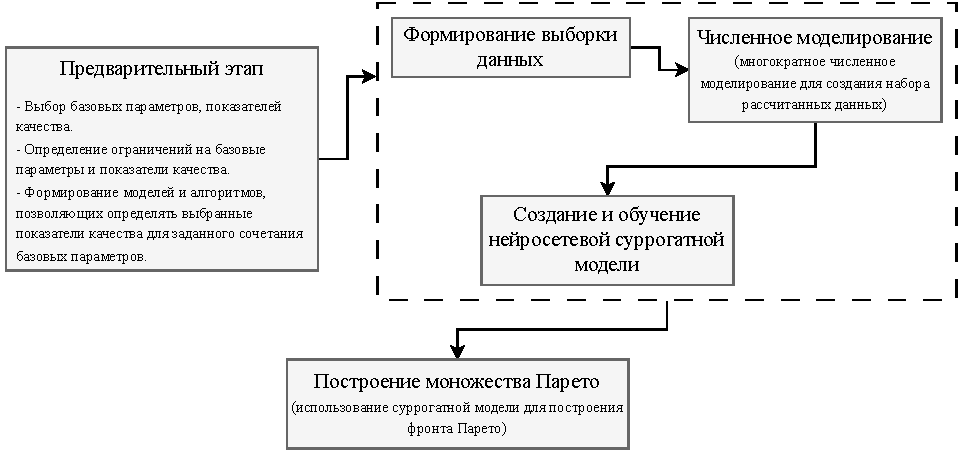
\includegraphics[width=\textwidth]{part5/диаграмма-процесса-формирования.pdf}
	\caption{Алгоритм построения фронта Парето}
	\label{fig:process-diagram}
	
\end{figure}

Для сокращения вычислительных затрат количество расчетных точек должно быть минимальным,
но достаточным для обеспечения необходимой точности замещающей модели.
Кроме того, точки должны быть равномерно распределены в пространстве параметров.

Были исследованы различные методы заполнения пространства параметров: равномерная сетка,
случайная выборка, метод латинского гиперкуба (Latin Hypercube Sampling, LHS) и метод Соболя.
Для количественной оценки равномерности покрытия пространства параметров был разработан метрический метод \cite{pub21},
основанный на сравнении удельного среднего расстояния между соседними точками.
Коэффициент Монте-Карло рассчитывался по формуле:

\begin{equation}
	I = \frac{0,5}{\sqrt{\frac{n}{A}}},
\end{equation}
где $n$ -- количество реальных точек, $A$ -- площадь области, в рассматриваемом случае $A = 1$.

Результаты расчета данного коэффициента для различных методов выборки представлены в таблице~\ref{tab:monte_carlo_coefficient}.

\begin{table}[ht]
	\centering
	\caption{Сравнение равномерности покрытия пространства параметров различными методами выборки}
	\label{tab:monte_carlo_coefficient}
    \small
	\begin{tabular}{lc}
		\midrule
		\textbf{Метод выборки}     & \textbf{Коэффициент Монте-Карло} \\
		\midrule
		Равномерная сетка          & 0,947                            \\
		Случайная выборка          & 1,024                            \\
		Метод латинского гиперкуба & 0,997                            \\
		Метод Соболя               & 0,980                            \\
		\midrule
	\end{tabular}
\end{table}

Как следует из таблицы, метод латинского гиперкуба (LHS) характеризуется
оптимальным значением коэффициента Монте-Карло,
что свидетельствует о наименьшей дисперсии расстояний между соседними точками и, соответственно,
о более равномерном заполнении пространства параметров. На рисунке \ref{fig:fill_field} представлены
примеры заполнения пространства параметров различными методами выборки.

\begin{figure}[ht]
	\centering
	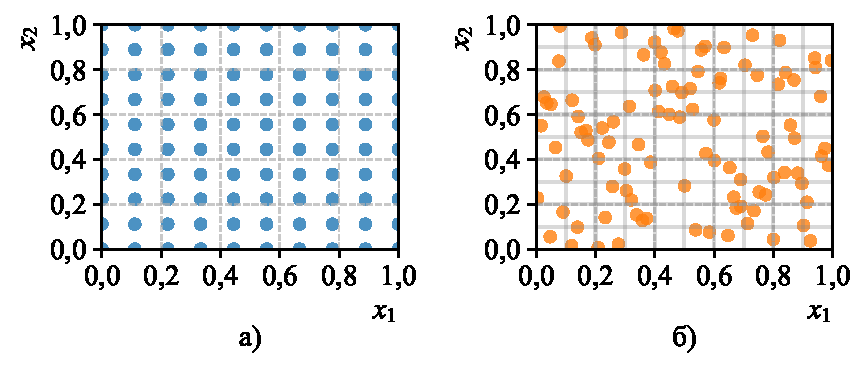
\includegraphics{part5/lhs_vs_grid.pdf}
	\caption{Заполнение пространства параметров различными методами выборки:\\
		a) равномерная сетка; б) метод латинского гиперкуба}
	\label{fig:fill_field}
\end{figure}

На основе проведенного анализа для формирования обучающей выборки данных при построении
суррогатных моделей был выбран метод латинского гиперкуба. 
Применение LHS позволило сформировать эффективную выборку из 2500 комбинаций базовых параметров, что
привело к снижению трудоемкости построения множества Парето и сокращению времени расчета на 48\%.
Использование выборки, сформированной методом латинского гиперкуба, обеспечило среднюю точность
замещающей суррогатной модели на уровне 91\% при максимальном отклонении 12\%.

Каждый эксперимент характеризуется вектором параметров $\mathbf{p}_i$ и соответствующим вектором
значений критериев оптимизации $\mathbf{J}_i = [AC_i, ITAE_i, SI_i]^T$. Общая обучающая выборка
представляет собой набор пар $\{(\mathbf{p}_i, \mathbf{J}_i)\}_{i=1}^N$, где $N$ -- общее число экспериментов.

Для повышения качества суррогатной модели проводится нормализация
входных и выходных данных с использованием стандартного масштабирования:

\begin{equation}
	\mathbf{p}_\text{норм} = \frac{\mathbf{p} - \boldsymbol{\mu}_p}{\boldsymbol{\sigma}_p},
\end{equation}
\begin{equation}
	\mathbf{J}_\text{норм} = \frac{\mathbf{J} - \boldsymbol{\mu}_J}{\boldsymbol{\sigma}_J},
\end{equation}
где $\boldsymbol{\mu}_p, \boldsymbol{\sigma}_p$ -- векторы средних значений и стандартных отклонений для параметров;
$\boldsymbol{\mu}_J, \boldsymbol{\sigma}_J$ -- векторы средних значений и стандартных отклонений для критериев.

Для повышения надёжности и точности предсказаний использовался ансамбль из нескольких суррогатных
моделей с различными начальными условиями. Каждая модель обучается минимизации взвешенной среднеквадратичной ошибки:

\begin{equation}
	\mathcal{L}(\mathbf{W}, \mathbf{b}) = \frac{1}{N} \sum_{i=1}^N w_i \cdot \|\mathbf{J}_{\text{норм},i} - f(\mathbf{p}_{\text{норм},i}; \mathbf{W}, \mathbf{b})\|_2^2,
\end{equation}
где $w_i$ -- весовой коэффициент для $i$-го образца;
$\mathbf{W}, \mathbf{b}$ -- обобщённые весовые матрицы и векторы смещения сети.

Для оптимизации параметров нейронной сети используется алгоритм AdamW с
начальной скоростью обучения $\eta = 10^{-3}$ и регуляризацией весов $\lambda = 10^{-4}$.
Для адаптивной настройки скорости обучения применяется циклический планировщик
(Cyclic Learning Rate Scheduler) с треугольным режимом изменения скорости.

Тренировка выполняется в течение заданного числа эпох (обычно 1000) с
мониторингом ошибки на валидационном наборе для предотвращения переобучения. Валидационный
набор формируется методом кросс-валидации (K-Fold Cross Validation) с K = 5.

Прогноз ансамбля моделей формируется как
среднее значение предсказаний отдельных моделей:

\begin{equation}
	\hat{\mathbf{J}}(\mathbf{p}) = \frac{1}{M} \sum_{m=1}^M f_m(\mathbf{p}),
\end{equation}
где $M$ -- количество моделей в ансамбле;
$f_m(\mathbf{p})$ -- предсказание $m$-й модели.

Для определения оптимальной архитектуры суррогатной модели проводится поиск гиперпараметров
с использованием байесовской оптимизации. В качестве оптимизируемых гиперпараметров рассматриваются:

\begin{itemize}
	\item Скорость обучения $\eta \in [10^{-4}, 10^{-2}]$
	\item Размерность первого скрытого слоя $h_1 \in [2, 64]$
	\item Размерность второго скрытого слоя $h_2 \in [2, 64]$
\end{itemize}

Целевой функцией оптимизации является средняя ошибка валидации при К-кратной перекрёстной
проверке. Байесовская оптимизация использует гауссовский процесс для построения вероятностной
модели зависимости ошибки валидации от гиперпараметров и последовательно выбирает точки в
пространстве гиперпараметров для максимизации ожидаемого улучшения (Expected Improvement).

После обучения ансамбля суррогатных моделей осуществляется поиск
Парето-оптимальных решений с использованием эволюционного алгоритма
многокритериальной оптимизации NSGA-III (Non-dominated Sorting Genetic Algorithm III).
Данный алгоритм для эффективного решения многокритериальных задач с большим числом
целевых функций.

Алгоритм NSGA-III основан на следующих принципах:
\begin{enumerate}
	\item Недоминируемая сортировка популяции решений на фронты.
	\item Использование опорных точек (reference points) для сохранения разнообразия решений вдоль фронта Парето.
	\item Эволюционные операторы селекции, скрещивания и мутации для исследования пространства решений.
\end{enumerate}

В результате проведения многокритериальной оптимизации были получены фронты Парето для 
позиционных пневмоприводов различной структуры, отражающие взаимосвязь между тремя
ключевыми критериями: точностью позиционирования ($AC$), интегральным критерием качества
($ITAE$) и интенсивностью переключений распределителей ($SI$).

\textbf{Парето-фронт для пневмопривода с модифицированным ПИД-регулятором и ШИМ.}
При исследовании ПИД-регулятора с ШИМ варьировались пять параметров: $K_p$, $K_i$, $K_d$,
частота ШИМ $f_{\text{ШИМ}}$ и коэффициент адаптивного торможения $K_{\text{т}}$.

Парето-фронт для ПИД-регулятора с ШИМ имеет относительно гладкую структуру без характерных
разрывов, что свидетельствует о плавном изменении свойств системы при варьировании параметров.
Минимальная точность позиционирования составляет 0,41 мм при значении динамического критерия $ITAE = 0,0305$ \si{\metre\per\second\square}
и интенсивности переключений $SI = 35$ переключений. При снижении требований к точности до 1,5 \si{\milli\metre} снижается
интенсивность переключений до $SI = 26$ при незначительном ухудшении динамики ($ITAE = 0,04$ \si{\metre\per\second\square}).

Характерной особенностью является небольшой диапазон изменения $ITAE$ (от 0,0298 до 0,0427 \si{\metre\per\second\square}) при значительном изменении
точности (от 0,41 до 2,57 мм), что указывает на ограниченные возможности ПИД-регулятора с ШИМ в
обеспечении высокой точности при сохранении приемлемых динамических характеристик.
На рисунке \ref{fig:pid_pareto} представлена поврерхность Пратео-фротна.
\begin{figure}[h]
	\centering
	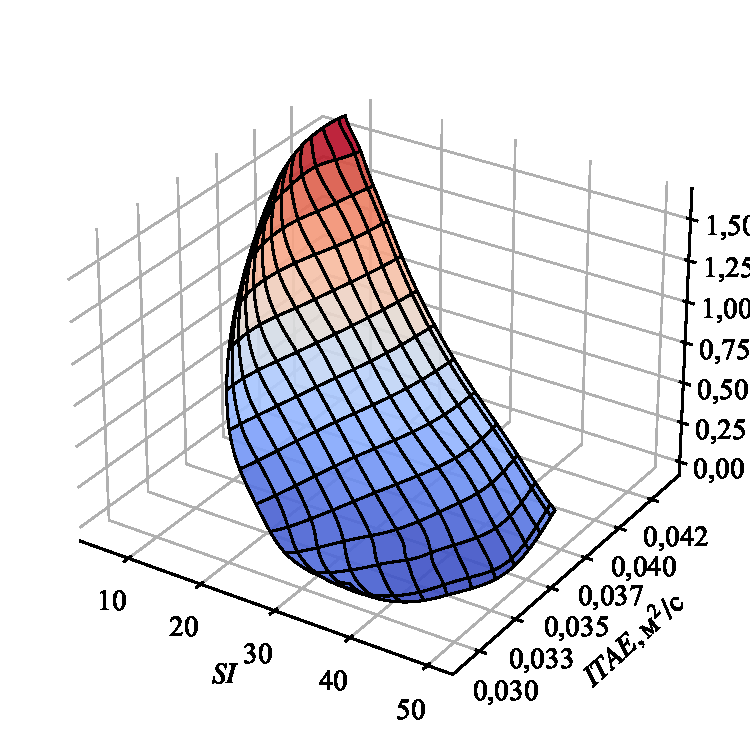
\includegraphics{part5/fronts/ПИД+ШИМ.pdf}
	\caption{Парето-фронт для ПИШ с ШИМ}
	\label{fig:pid_pareto}
\end{figure}

\textbf{Парето-фронты для пневмопривода с управлением в скользящих режимах.}
Исследование проводилось для комбинаций типов поверхностей скольжения (интегральная и терминальная)
и количества режимов управления (три, пять и семь).

Для трехрежимного управления с интегральной поверхностью (УСР-И-3) минимальная
точность составляет 0,8 мм при $ITAE = 0,051$ \si{\metre\per\second\square} и $SI = 20$
Характерной особенностью является разрыв в области $SI = 20$, указывающий на существование различных локально-оптимальных конфигураций.

Пятирежимное управление (УСР-И-5) обеспечивает значительное
улучшение: точность 0,36 мм при $ITAE = 0,033$ \si{\metre\per\second\square} и $SI = 5$.

Семирежимное управление с интегральной поверхностью (УСР-И-7) показывает
наилучшую точность 0,13 мм при $ITAE = 0,019$ \si{\metre\per\second\square} и $SI = 15$.

Трехрежимное управление с терминальной поверхностью (УСР-Т-3)
обеспечивает точность 0,31 мм, что в 2,5 раз лучше по сравнению с
интегральной поверхностью при том же количестве режимов. Пятирежимное
управление с терминальной поверхностью (УСР-Т-5) дает точность 0,28 мм при $ITAE = 0,019$
\si{\metre\per\second\square} и $SI = 10$.

Семирежимное управление с терминальной поверхностью (УСР-Т-7) обеспечивает
точность 0,13 мм при $ITAE = 0,024$ \si{\metre\per\second\square} и $SI = 15$.

Сравнительный анализ показывает, что терминальная поверхность обеспечивает более высокую точность
при малом числе режимов, но при увеличении числа режимов преимущество
становится менее выраженным. Для обоих типов поверхностей наиболее значительный скачок качества происходит при переходе от трех к пяти режимам.

На рисунке \ref{fig:scrolling_pareto} представлен Парето-фронт для УСР-И-3
\begin{figure}[h]
	\centering
	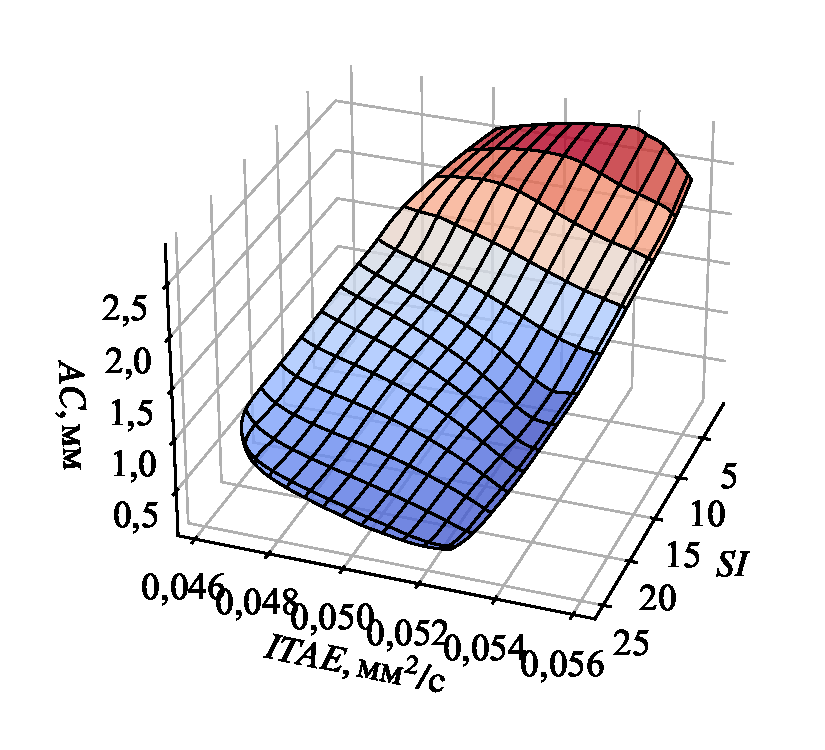
\includegraphics{part5/fronts/УСР-И-3.pdf}
	\caption{Парето-фронт для УСР-И-3}
	\label{fig:scrolling_pareto}
\end{figure}

\textbf{Парето-фронт для пневмопривода с нечетким управлением.}
При исследовании нечеткого управления варьировались формы
функций принадлежности, их расположение и конфигурация базы правил.

Парето-фронт для нечеткого регулятора имеет гладкую структуру.
Минимальная точность составляет 0,40 мм при $ITAE = 0,0551$ \si{\metre\per\second\square} и $SI = 23$,
что демонстрирует высокую эффективность нечеткого управления в обеспечении отличных динамических характеристик.

На рисунке \ref{fig:fuzzy_pareto} представлен Парето-фронт для нечеткого регулятора.
\begin{figure}[h]
	\centering
	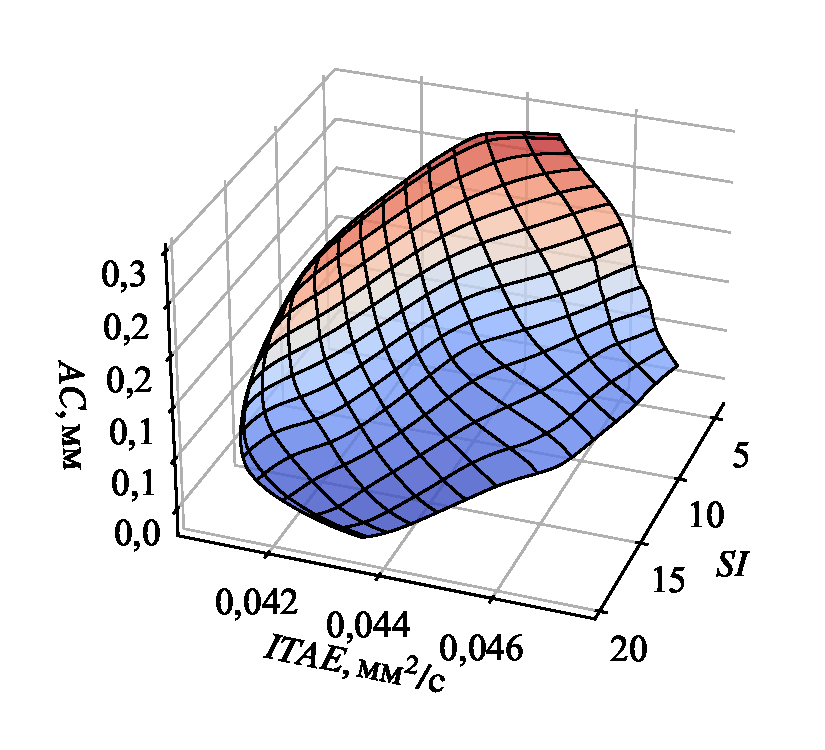
\includegraphics{part5/fronts/Нечеткий.pdf}
	\caption{Парето-фронт для нечеткого регулятора}
	\label{fig:fuzzy_pareto}
\end{figure}

\textbf{Парето-фронт для пневмопривода с прогнозным управлением.}
При исследовании прогнозного управления (MPC) варьировались горизонт прогноза,
горизонт управления, весовые коэффициенты целевой функции, параметры внутренней модели и шаг дискретизации.

Парето-фронт для MPC имеет ярко выраженную ступенчатую структуру с отчетливыми
кластерами решений. В области высокой точности (0,12 мм) наблюдается кластер
при $ITAE = 0,032$ \si{\metre\per\second\square} и $SI = 14$~--~$16$.

На рисунке \ref{fig:mpc_pareto} представлен Парето-фронт для MPC.
\begin{figure}[h]
	\centering
	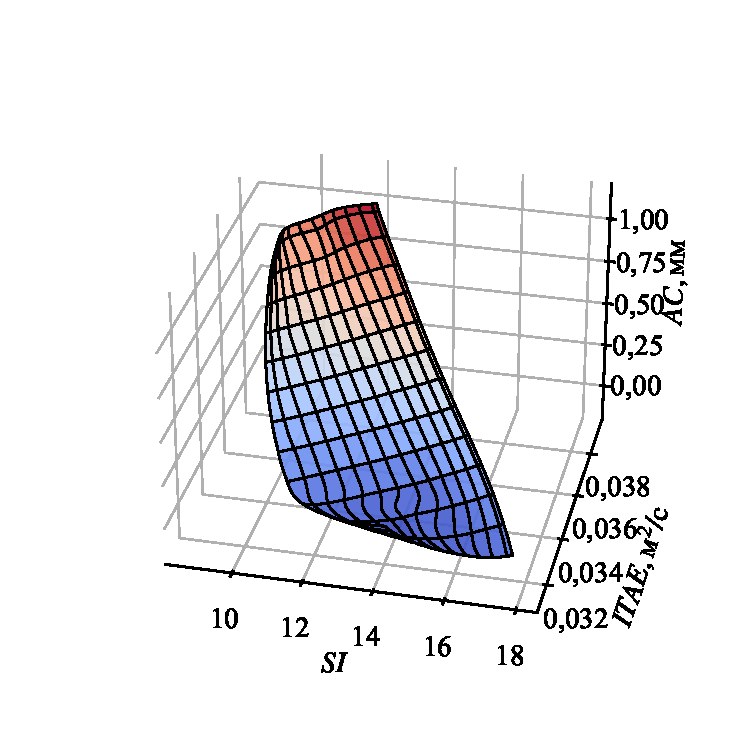
\includegraphics{part5/fronts/MPC.pdf}
	\caption{Парето-фронт для MPC}
	\label{fig:mpc_pareto}
\end{figure}

После формирования фронтов Парето для каждой конкурсной структуры
была проведена оценка точности построения границы Парето по суррогатной
модели. Для этого на сформированном фронте Парето равномерно выбирался
набор точек. Для каждой точки определялись значения вектора параметров,
соответствующего каждой точке. Далее производился расчет показателей качества
по исходной модели и сравнение результатов расчета со значениями,
соответствующими точкам на фронте Парето. 

Для количественной оценки погрешностей использовались следующие показатели:
\begin{enumerate}
	\item Относительная погрешность для каждого критерия:
	      \begin{equation}\label{eq:relative_error}
		      \delta_{\text{rel},i} = \frac{|y_i^{\text{факт}} - y_i^*|}{|y_i^*|} \cdot 100\%
	      \end{equation}

	\item Средняя относительная погрешность по всем критериям:
	      \begin{equation}\label{eq:mean_relative_error}
		      \delta_{\text{rel}} = \frac{1}{m} \sum_{i=1}^{m} \frac{|y_i^{\text{факт}} - y_i^*|}{|y_i^*|} \cdot 100\%
	      \end{equation}
	      где $m$ -- число критериев (в данном случае $m = 3$).

	\item Нормализованная абсолютная погрешность:
	      \begin{equation}\label{eq:normalized_absolute_error}
		      \delta_{\text{abs},i} = \frac{|y_i^{\text{факт}} - y_i^*|}{y_{i,\max} - y_{i,\min}} \cdot 100\%
	      \end{equation}

	\item Средняя нормализованная абсолютная погрешность:
	      \begin{equation}\label{eq:mean_normalized_absolute_error}
		      \delta_{\text{abs}} = \frac{1}{m} \sum_{i=1}^{m} \frac{|y_i^{\text{факт}} - y_i^*|}{y_{i,\max} - y_{i,\min}} \cdot 100\%
	      \end{equation}
\end{enumerate}

На рисунке~\ref{fig:verification_diagram} представлена лепестковая диаграмма
средних относительных погрешностей для конкурсных структур пневмопривода.
Из диаграммы видно, что наименьшая погрешность характерна для ПИД-регулятора с
ШИМ и нечеткого управления, что объясняется более плавной функциональной зависимостью
между параметрами и критериями в этих структурах. Наибольшая погрешность наблюдается
для семирежимного управления в скользящих режимах с терминальной поверхностью, что
связано с высокой нелинейностью и сложностью параметрической оптимизации этой структуры.

\begin{figure}[h]
	\centering
	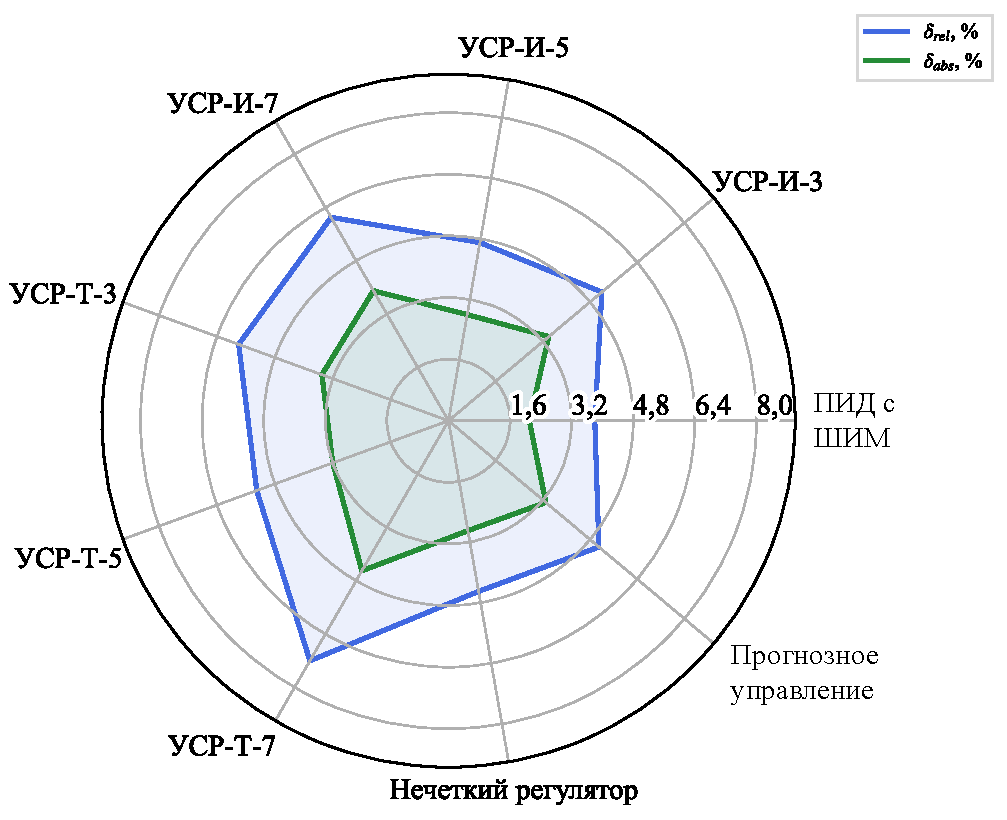
\includegraphics{part5/diagramm_error.pdf}
	\caption{Сравнение средних относительных погрешностей для различных конкурсных структур}
	\label{fig:verification_diagram}
\end{figure}

В таблице~\ref{tab:verification_results} приведены численные результаты
проверки применимости методики для различных управляющих структур.

\begin{table}[ht]
	\centering
	\caption{Результаты проверки применимости методики решения обратной задачи}
	\label{tab:verification_results}
	\small
	\begin{tabular}{lccc}
		\midrule
		\textbf{Метод управления} & $\delta_{\text{rel}}$,~\% & $\delta_{\text{abs}}$,~\% & \textbf{Максимальная погрешность}~\% \\
		\midrule
		ПИД-регулятор с ШИМ       & \num{3.8}                 & \num{2.1}                 & \num{9.2}                            \\
		УСР-И-3                   & \num{5.2}                 & \num{3.4}                 & \num{11.6}                           \\
		УСР-И-5                   & \num{4.7}                 & \num{2.8}                 & \num{10.3}                           \\
		УСР-И-7                   & \num{6.1}                 & \num{3.9}                 & \num{13.5}                           \\
		УСР-Т-3                   & \num{5.8}                 & \num{3.5}                 & \num{12.7}                           \\
		УСР-Т-5                   & \num{5.3}                 & \num{3.2}                 & \num{11.9}                           \\
		УСР-Т-7                   & \num{7.2}                 & \num{4.5}                 & \num{15.8}                           \\
		Нечеткий регулятор        & \num{4.5}                 & \num{2.9}                 & \num{10.8}                           \\
		Прогнозное управление     & \num{5.1}                 & \num{3.3}                 & \num{12.5}                           \\
		\midrule
	\end{tabular}
\end{table}

Для проверки применимости методики для различных требований к критериям проведен
дополнительный анализ, в ходе которого тестовые точки были разделены на группы по преобладающим требованиям:
\begin{itemize}
	\item Группа А -- приоритет точности позиционирования (малые значения $AC$).
	\item Группа Б -- приоритет динамических характеристик (малые значения $ITAE$).
	\item Группа В -- приоритет ресурсосбережения (малые значения $SI$).
	\item Группа Г -- сбалансированные требования ко всем критериям.
\end{itemize}

Результаты анализа показали, что методика наиболее эффективна для группы Г (сбалансированные требования),
где средняя относительная погрешность составила \num{4.2}\%. Для групп А, Б и В средние
относительные погрешности составили \num{5.7}\%, \num{4.9}\% и \num{5.5}\% соответственно.
Это свидетельствует о том, что методика обеспечивает приемлемую точность во всем диапазоне
требований, однако более эффективна при сбалансированных требованиях к критериям.